\documentclass{article}

\usepackage{polski}
\usepackage[utf8]{inputenc}

\usepackage{fancyhdr} % Required for custom headers
\usepackage{lastpage} % Required to determine the last page for the footer
\usepackage{extramarks} % Required for headers and footers
\usepackage[usenames,dvipsnames]{color} % Required for custom colors
\usepackage{graphicx} % Required to insert images
\usepackage{listings} % Required for insertion of code
\usepackage{courier} % Required for the courier font
\usepackage{lipsum} 
\usepackage{amsfonts}
\usepackage{amsthm}
\usepackage{hyperref}
\usepackage{tikz}
\usepackage{amsmath}
\usepackage{pdfpages}
\usepackage{mathtools}
\usepackage{enumitem}

\usepackage{amsthm}
\usepackage{epigraph}

\DeclareUnicodeCharacter{00A0}{ }

\makeatletter
\newenvironment{chapquote}[2][2em]
  {\setlength{\@tempdima}{#1}%
   \def\chapquote@author{#2}%
   \parshape 1 \@tempdima \dimexpr\textwidth-2\@tempdima\relax%
   \itshape}
  {\par\normalfont\hfill--\ \chapquote@author\hspace*{\@tempdima}\par\bigskip}
\makeatother

\newtheorem{thm}{Twierdzenie}
\newtheorem{remark}{Uwaga}
\newtheorem{lemat}{Lemat}
\newtheorem{wniosek}{Wniosek}
\newtheorem{definicja}{Definicja}
\newtheorem{ciekawostka}{Ciekawostka}
\newtheorem{przyklad}{Przykład}
\newtheorem{fakt}{Fakt}



\newenvironment{prooff}{\paragraph{Dowód:}}{\hfill$\square$}
\newenvironment{rozw}{\paragraph{Rozwiązanie:}}{\hfill}


\usepackage{inconsolata} % very nice fixed-width font included with texlive-full
\usepackage[usenames,dvipsnames]{color} % more flexible names for syntax highlighting colors
\usepackage{listings}

\lstset{
basicstyle=\small\ttfamily, 
columns=fullflexible, % make sure to use fixed-width font, CM typewriter is NOT fixed width
numbers=left, 
numberstyle=\small\ttfamily\color{Gray},
stepnumber=1,              
numbersep=10pt, 
numberfirstline=true, 
numberblanklines=true, 
tabsize=4,
lineskip=-1.5pt,
extendedchars=true,
breaklines=true,        
keywordstyle=\color{Blue}\bfseries,
identifierstyle=, % using emph or index keywords
commentstyle=\sffamily\color{OliveGreen},
stringstyle=\color{Maroon},
showstringspaces=false,
showtabs=false,
upquote=false,
texcl=true, % interpet comments as LaTeX
    literate={á}{{\'a}}1 {ã}{{\~a}}1 {é}{{<}}1,
inputencoding=utf8
}

\lstdefinelanguage{julia}
{
  keywordsprefix=\@,
  morekeywords={
    exit,whos,edit,load,is,isa,isequal,typeof,tuple,ntuple,uid,hash,finalizer,convert,promote,
    subtype,typemin,typemax,realmin,realmax,sizeof,eps,promote_type,method_exists,applicable,
    invoke,dlopen,dlsym,system,error,throw,assert,new,Inf,Nan,pi,im,begin,while,for,in,return,
    break,continue,macro,quote,let,if,elseif,else,try,catch,end,bitstype,ccall,do,using,module,
    import,export,importall,baremodule,immutable,local,global,const,Bool,Int,Int8,Int16,Int32,
    Int64,Uint,Uint8,Uint16,Uint32,Uint64,Float32,Float64,Complex64,Complex128,Any,Nothing,None,
    function,type,typealias,abstract
  },
  sensitive=true,
  morecomment=[l]{\#},
  morestring=[b]',
  morestring=[b]" 
}

% Margins
\topmargin=-0.45in
\evensidemargin=0in
\oddsidemargin=0in
\textwidth=6.0in
\textheight=9.0in
\headsep=0.25in

\linespread{1.1} % Line spacing

% Set up the header and footer
\pagestyle{fancy}
\lhead{\hmwkAuthorName} % Top left header
\rhead{\firstxmark} % Top right header
\lfoot{\lastxmark} % Bottom left footer
\cfoot{} % Bottom center footer
\renewcommand\headrulewidth{0.4pt} % Size of the header rule
\renewcommand\footrulewidth{0.4pt} % Size of the footer rule

\setlength\parindent{0pt} % Removes all indentation from paragraphs
%----------------------------------------------------------------------------------------
%	DOCUMENT STRUCTURE COMMANDS
%	Skip this unless you know what you're doing
%----------------------------------------------------------------------------------------

% Header and footer for when a page split occurs within a problem environment
\newcommand{\enterProblemHeader}[1]{
\nobreak\extramarks{#1}{#1 continued on next page\ldots}\nobreak
\nobreak\extramarks{#1 (continued)}{#1 continued on next page\ldots}\nobreak
}

% Header and footer for when a page split occurs between problem environments
\newcommand{\exitProblemHeader}[1]{
\nobreak\extramarks{#1 (continued)}{#1 continued on next page\ldots}\nobreak
\nobreak\extramarks{#1}{}\nobreak
}

\setcounter{secnumdepth}{0} % Removes default section numbers
\newcounter{homeworkProblemCounter} % Creates a counter to keep track of the number of problems

\newcommand{\homeworkProblemName}{}
\newenvironment{homeworkProblem}[1][Zadanie \arabic{homeworkProblemCounter}]{ % Makes a new environment called homeworkProblem which takes 1 argument (custom name) but the default is "Problem #"
\stepcounter{homeworkProblemCounter} % Increase counter for number of problems
\renewcommand{\homeworkProblemName}{#1} % Assign \homeworkProblemName the name of the problem
\section{\homeworkProblemName} % Make a section in the document with the custom problem count
\enterProblemHeader{\homeworkProblemName} % Header and footer within the environment
}{
\exitProblemHeader{\homeworkProblemName} % Header and footer after the environment
}

\newcommand{\problemAnswer}[1]{ % Defines the problem answer command with the content as the only argument
\noindent\framebox[\columnwidth][c]{\begin{minipage}{0.98\columnwidth}#1\end{minipage}} % Makes the box around the problem answer and puts the content inside
}

\newcommand{\homeworkSectionName}{}
\newenvironment{homeworkSection}[1]{ % New environment for sections within homework problems, takes 1 argument - the name of the section
\renewcommand{\homeworkSectionName}{#1} % Assign \homeworkSectionName to the name of the section from the environment argument
\subsection{\homeworkSectionName} % Make a subsection with the custom name of the subsection
\enterProblemHeader{\homeworkProblemName\ [\homeworkSectionName]} % Header and footer within the environment
}{
\enterProblemHeader{\homeworkProblemName} % Header and footer after the environment
}

\usepackage{listings} % Required for inserting code snippets
\usepackage[usenames,dvipsnames]{color} % Required for specifying custom colors and referring to colors by name

\definecolor{DarkGreen}{rgb}{0.0,0.4,0.0} % Comment color
\definecolor{highlight}{RGB}{255,251,204} % Code highlight color

% Create a command to cleanly insert a snippet with the style above anywhere in the document
\newcommand{\insertcode}[2]{\begin{itemize}\item[]\lstinputlisting[caption=#2,label=#1,style=Style1]{#1}\end{itemize}} % The first argument is the script location/filename and the second is a caption for the listing

%----------------------------------------------------------------------------------------
%	NAME AND CLASS SECTION
%----------------------------------------------------------------------------------------

\newcommand{\hmwkTitle}{Problem palaczy tytoniu} % Assignment title
\newcommand{\hmwkDueDate}{} % Due date
\newcommand{\hmwkClass}{Systemy operacyjne} % Course/class
\newcommand{\hmwkClassTime}{} % Class/lecture time
\newcommand{\hmwkClassInstructor}{} % Teacher/lecturer
\newcommand{\hmwkAuthorName}{Bartosz Bednarczyk - obowiązkowe zadanie z systemów operacyjnych} % Your name

%----------------------------------------------------------------------------------------

\begin{document}

\title{Problem palaczy tytoniu}
\date{\today}
\author{Bartosz Bednarczyk}

\maketitle

%%%%%%%%%%%%%%%%%%%%%%%%%%%%%%%%%%%%%%%%%%%%%%%%%%%%%%%%%%%%%%%%%%%%%%%%%%%

\subsection*{Wymagania techniczne}

Rozwiązanie powinno być napisane w języku C i kompilować się bez błędów z opcjami \textbf{-std=gnu99 -Wall -Wextra} kompilatorem \textbf{gcc} lub  \textbf{clang} w systemie \textbf{Linux}. Do rozwiązania musi być dostarczony plik \textbf{Makefile} tak, aby po wywołaniu polecenia \textbf{make} otrzymać pliki binarne, a polecenie \textbf{make clean} powinno zostawić w katalogu tylko pliki źródłowe.

\subsection*{Treść zadania}

\begin{center}
\begin{tikzpicture}
\node [draw={black}, fill=black!10, very thick, rectangle, rounded corners, inner sep=12pt, inner ysep=12pt] (box){%
    \begin{minipage}{.9\textwidth}

Przypuśćmy, że istnieją trzy procesy palaczy i jeden proces agenta. Każdy z palaczy na okrągło robi papierosy i je pali. Zrobienie i zapalenie papierosa wymaga tytoniu, bibułki i zapałek. Każdy palacz posiada nieskończoną ilość wyłącznie jednego typu zasobu, tj. pierwszy ma tytoń, drugi bibułki, a trzeci zapałki. Agent kładzie na stole dwa składniki. Palacz, który ma brakujący składnik, podnosi ze stołu resztę, skręca papierosa i go zapala. Agent czeka, aż palacz skończy palić, po czym powtarza cykl.

    \end{minipage}
};
\node[fill={black}, text=white, rounded corners, right=10pt] at (box.north west) {Treść zadania};
\end{tikzpicture}
\end{center}

\subsection*{Historia problemu}

Problem palaczy tytoniu został po raz pierwszy przedstawiony przez Suhasa Patila w 1971 roku, który uważał, że~nie da się go rozwiązać przy pomocy semaforów. Krótko opiszę trzy wersje problemu.\\

W pierwszej wersji Patil zakładał dodatkowe ograniczenie na rozwiązanie. Po pierwsze, nie wolno było modyfikować kodu agenta. Jeśli agent miałby reprezentować system operacyjny, to sensownie jest założyć, że nie chcemy go zmieniać z każdą nową aplikacją. Drugim ograniczeniem jest to, że nie możemy używać instrukcji warunkowych lub tablic semaforów. Przy takich ograniczeniach problem nie może być rozwiązany, ale jak Pernas wskazuje, drugie ograniczenie jest dość sztuczne. Z ograniczeniami jak te, wiele problemów synchronizacyjnych okazuje się być nierozwiązywalne.\\

W drugiej, ciekawszej wersji problemu, pomijamy drugie z powyższych założeń.\\

Trzecia wersja problemu polega na tym, że agent informuje palacza o możliwości zrobienia papierosa. Ten przypadek jest niepraktyczny, gdyż wymaga od agenta informacji na temat innych palaczy. Dodatkowo założenie o składnikach papierosów jest wtedy nieistotne. Ponadto, przedstawiona wersja jest zbyt łatwa, by nadawać się na pracownię z~systemów operacyjnych.

\pagebreak

\subsection*{Potencjalne problemy}

Podczas rozwiązywania zadania można napotkać się z następującymi problemami:

\begin{itemize}
\item zabranie składników ze stołu przez dwóch różnych palaczy; 
\item kelner nie czeka, aż palacz skończy palić papierosa.
\end{itemize}

\subsection*{Rozwiązanie}

Rozwiązanie umieszczone jest w katalogu ,,Palacze" dołączonym do sprawozdania.\\ Opis algorytmu i szczegóły implementacji można łatwo wyczytać z kodu źródłowego.

Przykładowy wynik uruchomienia programu możemy zaobserwować na poniższym zdjęciu:

\begin{figure}[h!]
\centering
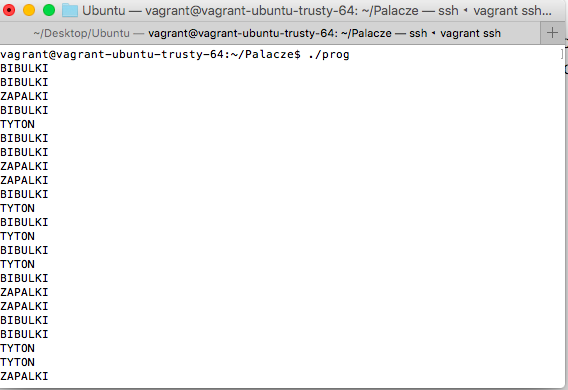
\includegraphics[scale=0.4]{zrzut_ekranu}	
\end{figure}

Słowa ,,BIBUŁKI'', ,,TYTON'', ,,ZAPALKI'' oznaczają, że palacz, który posiada wypisany przez program zasób, zapalił papierosa. Program działa do czasu, aż nie zostanie sam wyłączony przez użytkownika.

\subsection{Testy}

Program uruchamiany był wielokrotnie i podczas jego uruchomień zaobserwowałem, że działa on płynnie i bez opóźnień. Sugeruje to, że nie dochodzi do zakleszczeń procesów.\\

Przeprowadziłem również badanie polegające na porównaniu liczby wystąpień odpowiednich wyrazów. Po zatrzymaniu programu, wypisał on $11052$ wyrazy. Spośród nich 3660 to ,,TYTON'', 3712 to ,,ZAPALKI'', a 3680 to ,,BIBULKI''. Sugeruje to, iż rozłożenie aktywności różnych palaczy w czasie jest w miarę równomierne.  

\end{document}